% !TEX program = pdflatex
\documentclass[aspectratio=169, 11pt]{beamer}

\usetheme{default}
\usecolortheme{default}
\setbeamertemplate{navigation symbols}{}
\setbeamertemplate{footline}[frame number]
\setbeamertemplate{frametitle}{\vspace{0.5em}\textbf{\insertframetitle}}

\usepackage{amsmath,amssymb}
\usepackage{graphicx}
\usepackage{booktabs}
\usepackage{colortbl}
\usepackage{xcolor}
\usepackage{pgfpages}

% Notes on second screen for Pympress presenter view.
% Comment out for a standard single-page PDF.
\setbeameroption{show notes on second screen=right}

\graphicspath{{../}}

\definecolor{resultbg}{HTML}{E8F5E9}
\definecolor{newbg}{HTML}{FFF9C4}
\definecolor{proofbg}{HTML}{E3F2FD}

\title{Week 4 Update}
\author{Michael Fang}
\date{March 2026}

\begin{document}

%----------------------------------------------------------------------
\begin{frame}
\centering
\vspace{2em}
{\Large\textbf{Week 4 Update}}

\vspace{1em}
Michael Fang

\vspace{0.5em}
March 2026
\end{frame}
\note{
Topics this week:
\begin{itemize}
  \item Why $\alpha$ can't exceed 3 (rank-dependent bound)
  \item What controls the $\bar\Lambda$ ranking
  \item URL sweep, $g_2$-invariant patterns, metallic chain figures
  \item Yuan-Torquato improved spreadability for BT
  \item 138 $|\det M|{=}2$ chains
\end{itemize}
}

%----------------------------------------------------------------------
\begin{frame}[shrink=3]{Recap}

\small
\textbf{Last week:} proved $2{<}\alpha{<}3$ gap for $|\det M|{=}1$ matrices,
found first $|\det M|{=}2$ example at $\alpha=2.071$,
Silver $\bar\Lambda=1/4$, metallic-mean sequence approaching ${\sim}1/3$.

\medskip
\normalsize
Since last meeting:
\begin{itemize}
  \item Worked out why $\alpha$ can't exceed 3 for $|\det M|{=}1$ substitutions
  \item Understood what determines the $\bar\Lambda$ ranking
  \item Swept URL $\bar\Lambda(a)$ across $a \in [0, 2]$
  \item Looked into $g_2$-invariant patterns from Torquato \& Stillinger (2003)
  \item Generated metallic-mean tile visualizations for $n = 1$ through $10$
  \item Extended metallic-mean $\bar\Lambda$ to $n = 100$
  \item Implemented Yuan-Torquato (2026) improved spreadability fitting
  \item Computed $\bar\Lambda$ for all 138 $|\det M|{=}2$ chains with $\alpha\in(2,3)$
\end{itemize}

\end{frame}
\note{
Week 3 catalog for reference:
\begin{tabular}{lccc}
Pattern & $\alpha$ & $\bar\Lambda$ \\
\hline
Integer Lattice & --- & $1/6$ \\
Fibonacci & 3 & 0.201 \\
Silver & 3 & $1/4$ \\
Bronze & 3 & 0.282 \\
URL ($a{=}1$) & 2 & $1/3$ \\
BT & 1.545 & 0.377 \\
\end{tabular}
}

%----------------------------------------------------------------------
\begin{frame}{Why $\alpha$ can't exceed 3}

For a rank-$r$ substitution matrix with $|\det M|=1$ and all $|\lambda_i|<1$ for $i\geq 2$:
\[
  \underbrace{\lambda_1\prod_{i=2}^{r}|\lambda_i|}_{=\,|\det M|\,=\,1}
  \;\leq\; \lambda_1\,|\lambda_2|^{r-1}
  \quad\Rightarrow\quad
  |\lambda_2| \;\geq\; \lambda_1^{-1/(r-1)}
\]
Substituting into $\alpha = 1 - 2\ln|\lambda_2|/\ln\lambda_1$:
\[
  \boxed{\;\alpha \;\leq\; 1 + \frac{2}{r-1}\;}
\]

\medskip
\centering
\begin{tabular}{ccl}
\toprule
Rank $r$ & $\alpha_{\max}$ & Example \\
\midrule
2 & $\mathbf{3}$ & all metallic means (Fibonacci, Silver, \ldots) \\
3 & 2 & 504 cubic matrices with complex pair \\
4 & $5/3$ & \\
$r\to\infty$ & $\to 1^+$ & \\
\bottomrule
\end{tabular}

\end{frame}
\note{
The bound is tight for rank 2: metallic means saturate it.
For rank 3: saturated by the complex-pair case ($\alpha = 2$ exactly).

Higher rank $\to$ more eigenvalues sharing the determinant constraint
$\to$ $|\lambda_2|$ forced larger $\to$ $\alpha$ forced smaller.

For $|\det M| > 1$, the bound generalizes to
$\alpha \leq 1 + \frac{2}{r-1}\bigl(1 - \frac{\ln|\det M|}{\ln\lambda_1}\bigr)$.
}

%----------------------------------------------------------------------
\begin{frame}{What determines the $\bar\Lambda$ ranking?}

$\bar\Lambda$ measures residual large-scale density fluctuations.\\
More disorder $\to$ larger $\bar\Lambda$.

\medskip
\begin{itemize}
  \item \textbf{Lattice} (perfect order): $\bar\Lambda = 1/6$, global minimum

  \item \textbf{Metallic means} (tile disparity): as $n$ grows,
        $L/S = \mu_n$ increases, short tiles become rare defects\\
        $\Rightarrow$ $\bar\Lambda$ increases: $0.201 \to 0.250 \to \cdots \to {\sim}1/3$

  \item \textbf{URL} (displacement amplitude):
        $\bar\Lambda = (1+a^2)/6$, exact.
        Larger $a$ = more displacement = more disorder

  \item \textbf{Stealthy} (constraint strength):
        $\bar\Lambda \approx 1/(\pi^2\chi)$.
        Smaller $\chi$ = fewer constrained modes

  \item \textbf{BT} (slow $S(k)$ suppression):
        $\alpha = 1.545$, close to Class~II;
        large $|\lambda_2| = 0.802$ $\to$ $\bar\Lambda = 0.377$
\end{itemize}

\end{frame}
\note{
All our patterns fit a single story:
more structural disorder = larger $\bar\Lambda$.

The metallic-mean sequence is the clearest demonstration:
a continuous family with $\bar\Lambda$ increasing
from $0.201$ (Fibonacci) toward ${\sim}1/3$.
}

%----------------------------------------------------------------------
\begin{frame}{URL: $\bar\Lambda(a)$ for intermediate displacements}

\centering
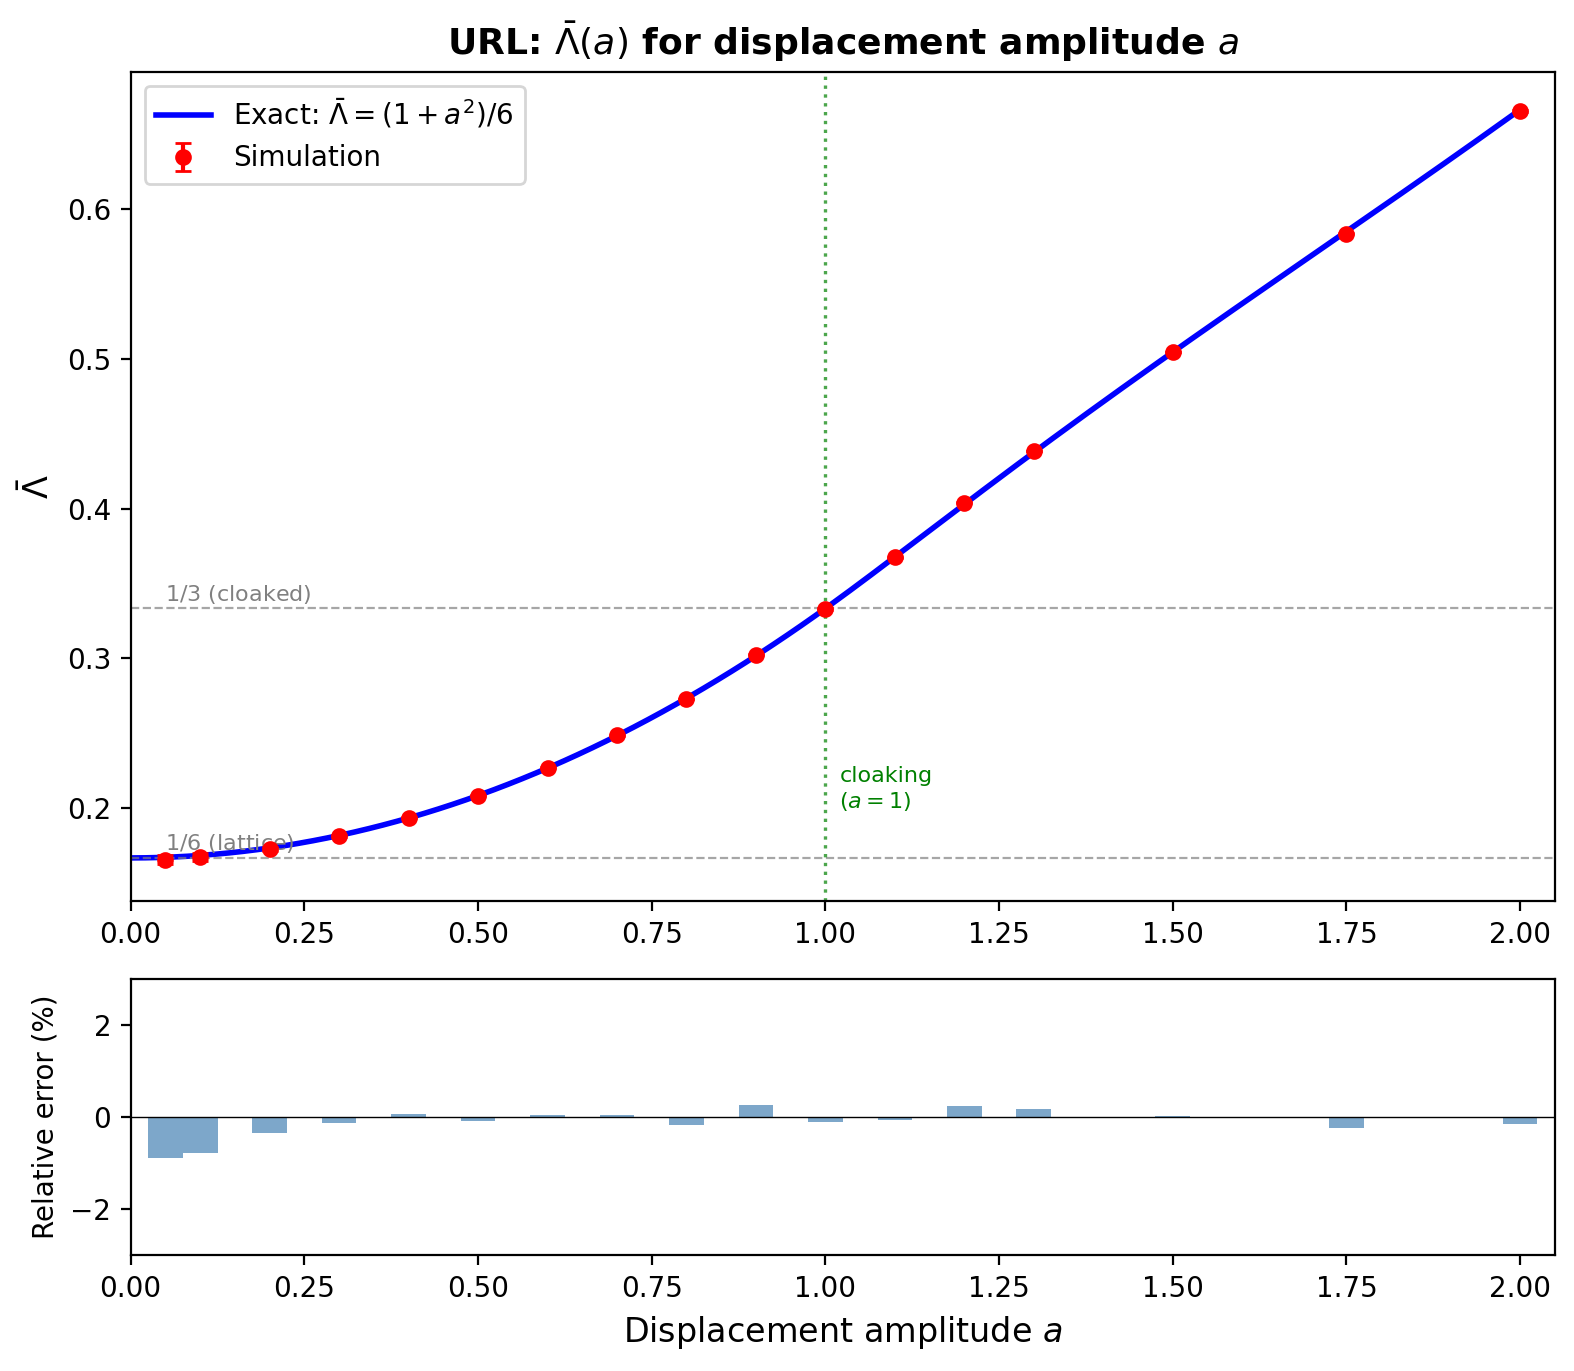
\includegraphics[height=0.68\textheight]{figures/fig_url_sweep.png}

\vspace{0.2em}
\small
17 values of $a \in [0.05,\, 2.0]$, $N = 50{,}000$.
All match the exact formula $\bar\Lambda = (1+a^2)/6$ to $< 1\%$.
At $a = 1$: Bragg peaks vanish (cloaking), $\bar\Lambda = 1/3$.

\end{frame}
\note{
Cloaking: the displacement form factor
$\tilde f(k) = \sin(\pi k a)/(\pi k a)$ vanishes at all non-zero
reciprocal lattice vectors when $a$ is an integer.

At $a=1$: $\bar\Lambda = 1/3$, close to where the metallic-mean sequence appears to be heading.

For $a > 1$, displacement intervals overlap. $\bar\Lambda$ continues
to increase: $\bar\Lambda(2) \approx 0.667$ at the second cloaking event.

Klatt et al.\ (2020) derived the formula analytically.
}

%----------------------------------------------------------------------
\begin{frame}{$g_2$-invariant patterns}

From Torquato \& Stillinger (2003): a $g_2$-invariant process has a fixed
pair correlation $g_2(r)$ across a range of densities.
At terminal density: $S(0) = 0$ (hyperuniform).

\medskip
\centering
\begin{tabular}{llc}
\toprule
\textbf{Pattern} & \textbf{Construction} & $\bar\Lambda$ \\
\midrule
Step-function $g_2$ & hard rods at close packing & $1/6$ (lattice) \\
Lattice-gas & one point uniform per cell & $1/3$ (= URL $a{=}1$) \\
Gauss.\ shuffled, $\sigma{=}0.1$ & $\mathcal{N}(0, 0.01)$ per site & $0.20 \pm 0.02$ \\
Gauss.\ shuffled, $\sigma{=}0.2$ & $\mathcal{N}(0, 0.04)$ per site & $0.250 \pm 0.007$ \\
Gauss.\ shuffled, $\sigma{=}0.3$ & $\mathcal{N}(0, 0.09)$ per site & $0.342 \pm 0.001$ \\
\bottomrule
\end{tabular}

\medskip
\small
The lattice-gas is just URL $a{=}1$ with a phase offset.
Gaussian shuffled lattice at $\sigma{=}0.1$ matches Fibonacci;
$\sigma{=}0.2$ matches Silver ($1/4$).

\end{frame}
\note{
The 1D $g_2$-invariant processes all reduce to perturbed lattices.
``Lattice-gas'': tessellate line into unit cells, place one point
uniformly in each. This is $j + U(0,1)$ vs.\ URL's $j + U(-1/2, 1/2)$.

The Gaussian results are interesting: deterministic quasicrystals
(Fibonacci, Silver) happen to match specific Gaussian displacements.
The structures are completely different, but the large-scale fluctuations
are the same.
}

%----------------------------------------------------------------------
\begin{frame}{Metallic-mean tile sequences}

\centering
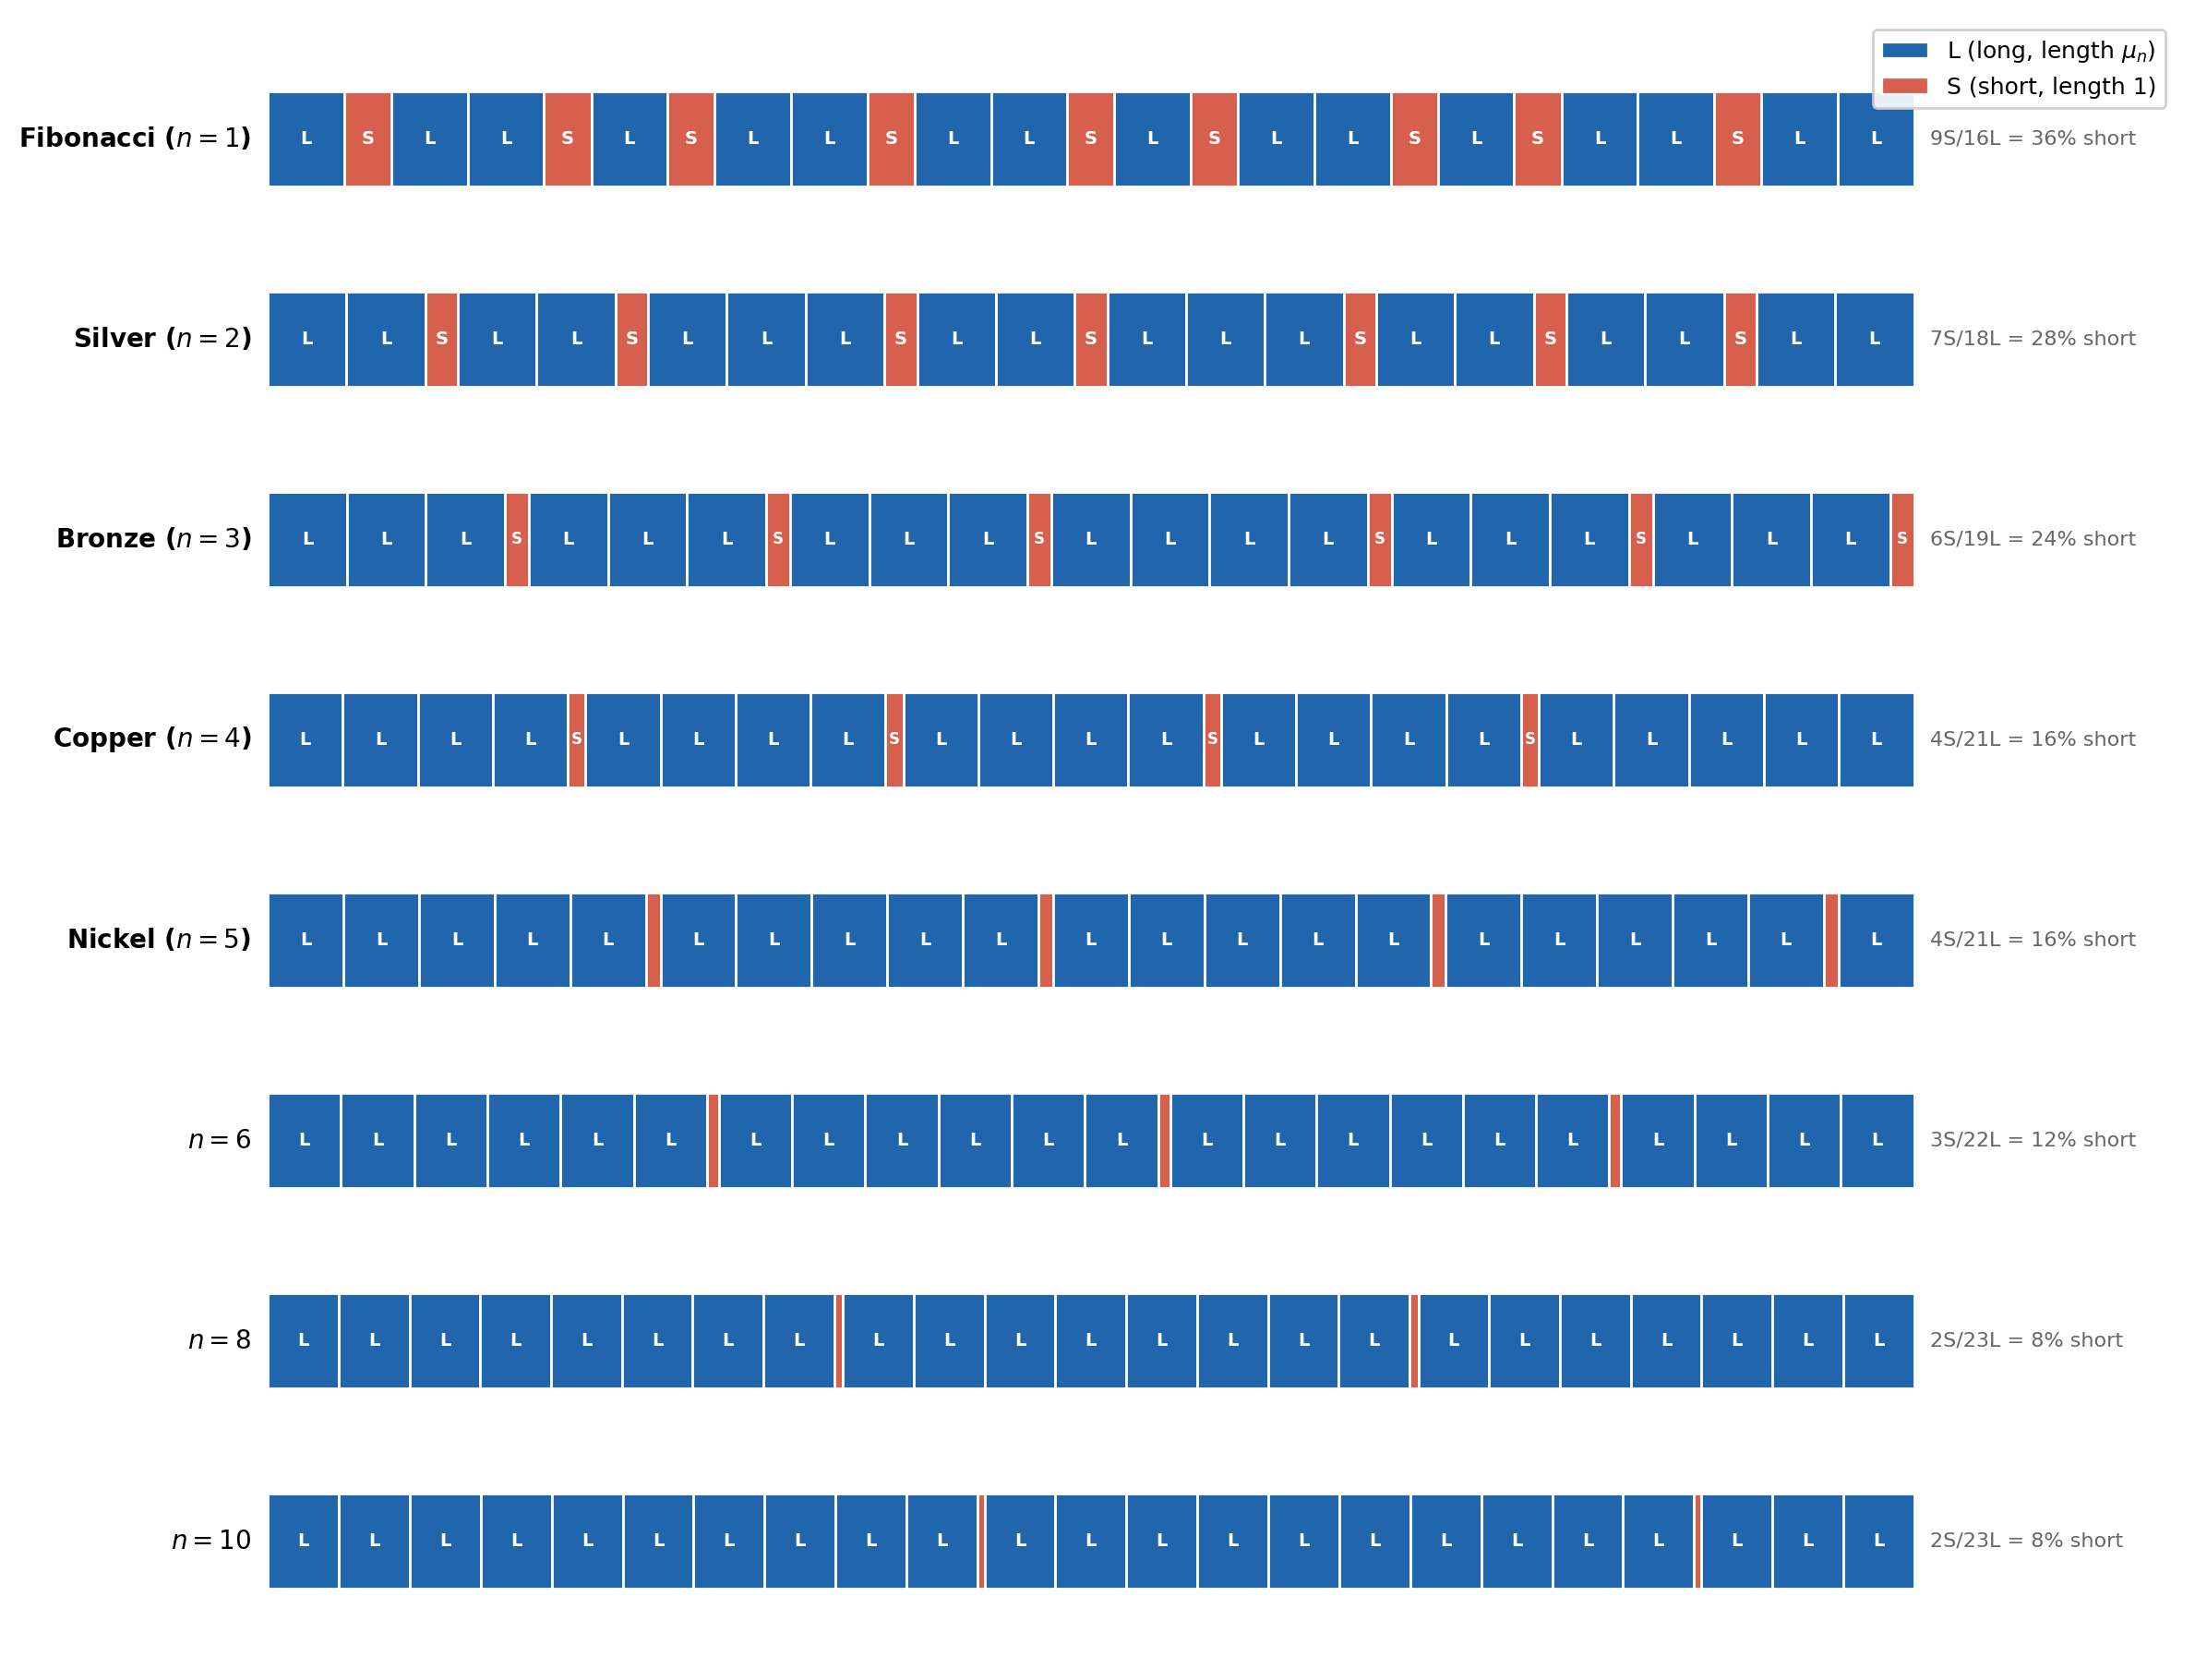
\includegraphics[width=0.88\linewidth,height=0.65\textheight,keepaspectratio]{figures/fig_metallic_tiles_extended.png}

\vspace{0.3em}
\small
25 tiles per chain. Short tiles (red) become rarer as $n$ increases:
$36\%$ at $n{=}1$ (Fibonacci) $\to$ $8\%$ at $n{=}10$.\\[0.2em]
For large $n$, the chain is nearly a lattice with rare short-tile defects.

\end{frame}
\note{
Rules: $S \to L$, $L \to L^n S$.

$n=1$ (Fibonacci): $S \to L$, $L \to LS$. Balanced quasi-periodic mix.

$n=10$: $L \to LLLLLLLLLLS$. Almost all L tiles, rare S defects.

S fraction $= 1/\mu_n \to 0$ as $n\to\infty$.
The chain approaches a lattice with rare quasi-random defects.
If the limit is $1/3$, this would match URL $a = 1$.
}

%----------------------------------------------------------------------
\begin{frame}{Metallic-mean $\bar\Lambda$ extended to $n = 100$}

\begin{columns}[c]
\begin{column}{0.55\textwidth}
\centering

\includegraphics[width=\linewidth]{figures/fig_metallic_convergence.png}
\end{column}
\begin{column}{0.43\textwidth}
\centering
\small
\begin{tabular}{rcc}
\toprule
$n$ & $\bar\Lambda$ & $1/3 - \bar\Lambda$ \\
\midrule
1 (Fib) & 0.199 & 0.134 \\
2 (Silv) & 0.250 & 0.083 \\
5 & 0.310 & 0.024 \\
10 & 0.327 & 0.007 \\
20 & 0.332 & 0.002 \\
50 & 0.334 & $-$0.001 \\
100 & 0.335 & $-$0.002 \\
\bottomrule
\end{tabular}

\vspace{0.5em}
\normalsize
$n \geq 50$: slightly above $1/3$\\
and still drifting up.
\end{column}
\end{columns}

\vspace{0.3em}
\centering
\colorbox{newbg}{\parbox{0.85\linewidth}{\centering
  Approaches $1/3$ from below through $n = 20$,
  but large-$n$ values ($n \geq 50$) overshoot.\\
  Cannot confirm convergence to exactly $1/3$ from this data.
}}

\end{frame}
\note{
Extended from $n=20$ (last week) to $n=100$.

$n = 1\ldots20$: monotone increasing toward $1/3$ from below.
$n = 50$: $0.334$, $n = 100$: $0.335$ --- both slightly above $1/3 = 0.333$.

Three possibilities:
1. True limit is $1/3$, overshoots are noise (error bars $\sim 0.005$,
   but may be underestimated at large $n$ where only 2 substitution
   iterations fit in $N = 300$k).
2. True limit is slightly above $1/3$.
3. Doesn't converge (unlikely given the smooth trend for $n \leq 20$).

The $n = 1\ldots20$ data strongly suggests a limit near $1/3$,
but higher-precision measurements at large $n$ are needed to
determine whether it's exactly $1/3$.

Figure shows the original $n = 1\ldots20$ data only.
}

%----------------------------------------------------------------------
\begin{frame}[shrink=2]{Yuan-Torquato improved spreadability}

\centering
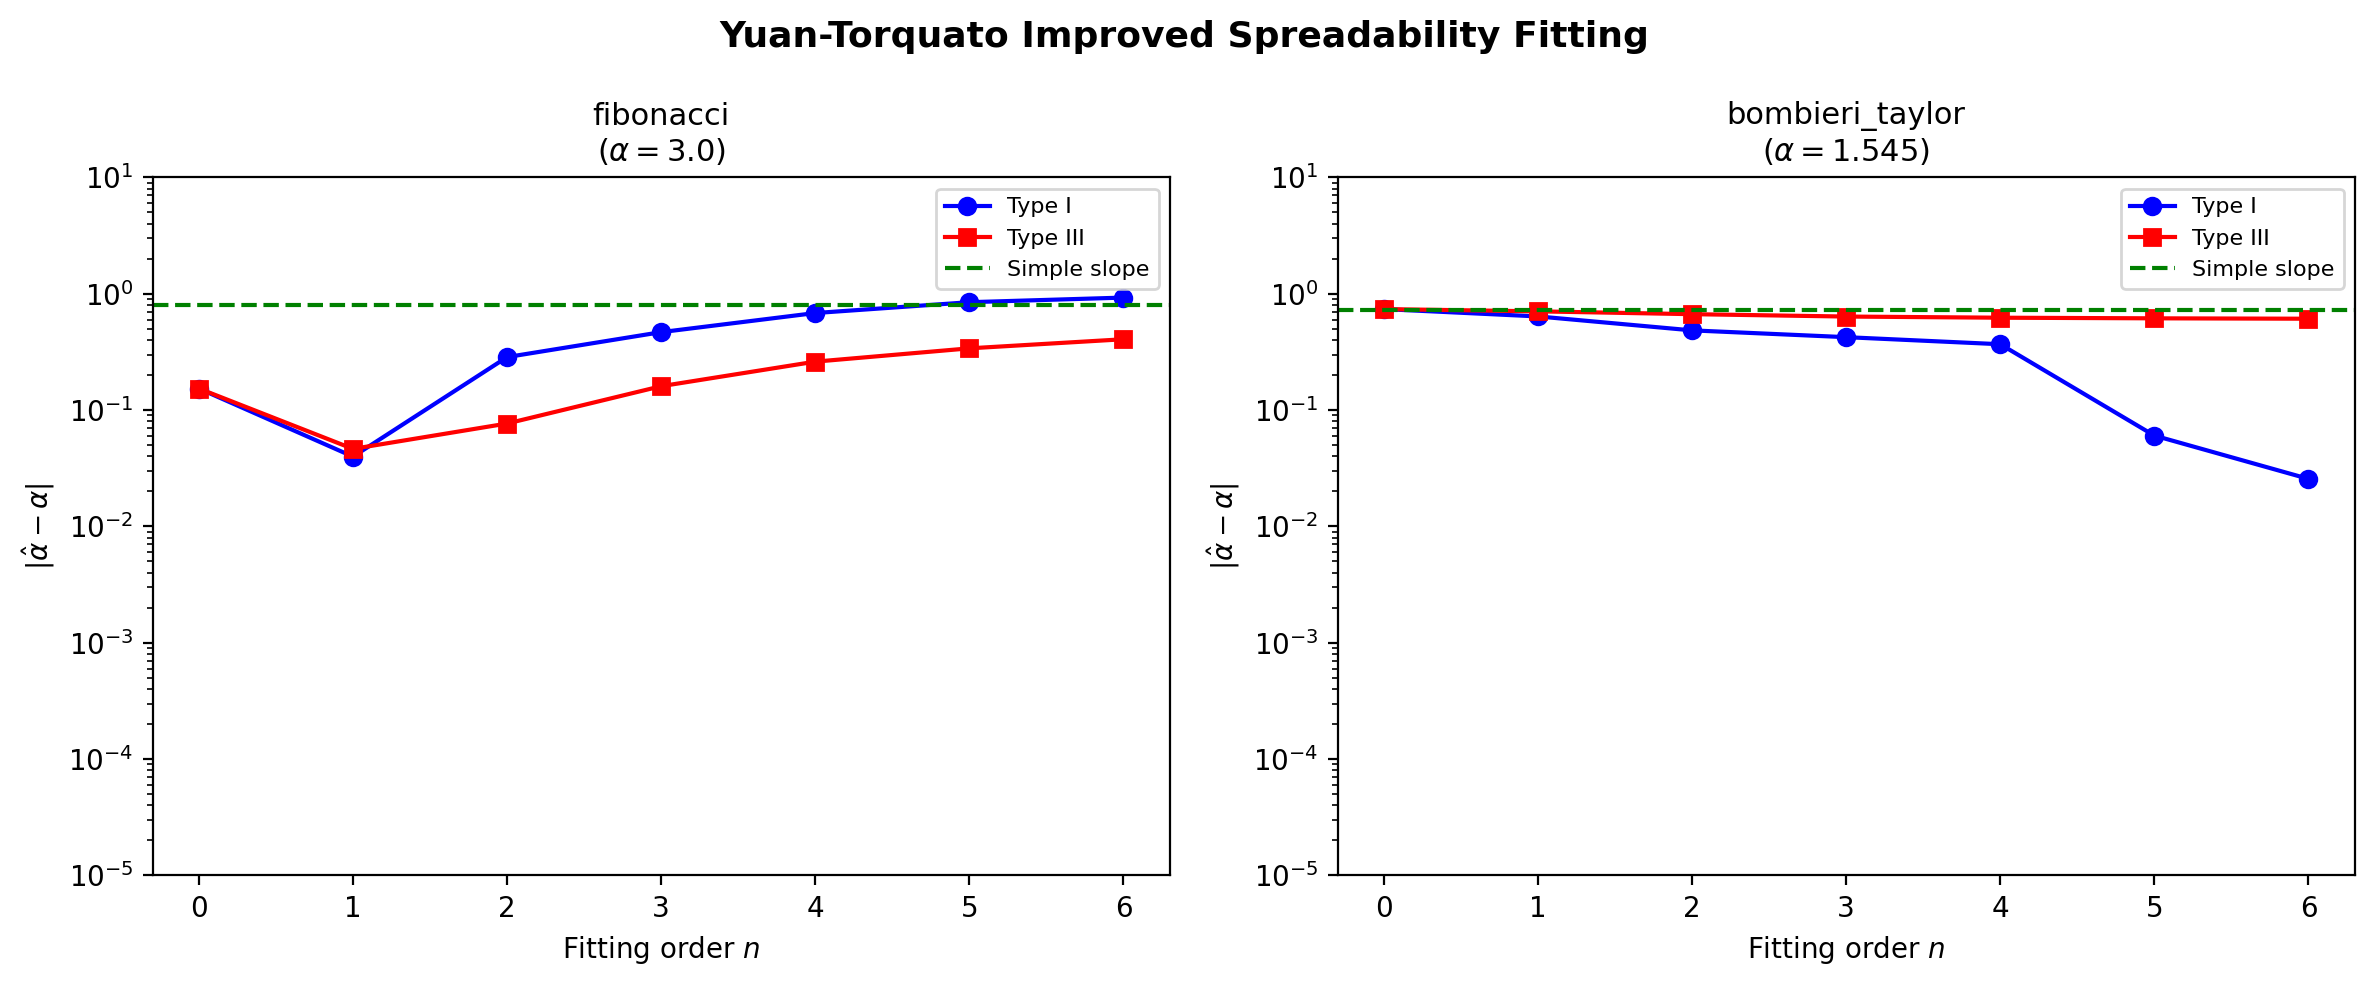
\includegraphics[width=0.78\linewidth]{figures/fig_yuan_spreadability.png}

\vspace{0.3em}
\small
\begin{tabular}{llcc}
\toprule
\textbf{Chain} & \textbf{Method} & $\hat\alpha$ & Error \\
\midrule
Fibonacci ($\alpha{=}3$) & Simple log-slope & 2.19 & 27\% \\
                         & Type~I, order 1 & 3.04 & 1.3\% \\
\midrule
BT ($\alpha{=}1.545$) & Simple log-slope & 2.27 & 47\% \\
                       & Type~I, order 6 & 1.57 & 1.7\% \\
\bottomrule
\end{tabular}

\vspace{0.2em}
\small
BT: first accurate $\alpha$ from moderate-time spreadability ($t \leq 10^6$).
Previously needed $t > 10^8$.

\end{frame}
\note{
Yuan \& Torquato (2026), arXiv:2602.17873.

They add higher-order correction terms to the long-time
asymptotic expansion of $s^{ex}(t)$.

Type I: $\ln[s^{ex}] = -(d+\alpha)/2 \cdot \ln t + \ln(\sum C_{i/2}\, t^{-i/2})$.
Fitting order $n$ = number of correction terms.

For BT: correction terms from large $|\lambda_2| = 0.802$ are big,
so higher-order fits help a lot.

For Fibonacci: $\alpha = 3$ (integer), dense Bragg peaks cause
the expansion to diverge at order $> 1$.

Their Section VI notes that quasicrystals with dense Bragg peaks
are not covered by the regular expansion theory.
The method is designed for disordered media.
}

%----------------------------------------------------------------------
\begin{frame}[shrink=3]{All $|\det M|{=}2$ chains with $\alpha \in (2,3)$}

Searched all $2\times2$ matrices with $|\det M| = 2$,\;
$|\lambda_2| < 1$,\; row sums $\leq 10$:

\medskip
\begin{columns}[c]
\begin{column}{0.52\textwidth}
\centering
\small
\begin{tabular}{ccc}
\toprule
$\alpha$ & Chains & $\bar\Lambda$ range \\
\midrule
2.071 & 12 & $[0.32,\; 2.01]$ \\
2.087 & 10 & $[0.34,\; 1.57]$ \\
2.175 & 18 & $[0.32,\; 3.36]$ \\
2.271 & 16 & $[0.34,\; 3.76]$ \\
2.301 & 18 & $[0.33,\; 4.05]$ \\
2.362 & 12 & $[0.34,\; 4.80]$ \\
2.393 &  4 & $[0.34,\; 5.08]$ \\
\bottomrule
\end{tabular}
\end{column}
\begin{column}{0.46\textwidth}
\textbf{138 chains total}\\
12 distinct $\alpha$ values\\
(7 shown)\\[0.3em]
$\alpha \in [2.07,\, 2.39]$\\[0.5em]
$\bar\Lambda$ varies by factors of\\
5--15 \emph{within each $\alpha$ group}\\[0.5em]
\colorbox{newbg}{\parbox{0.9\linewidth}{\small
  $\alpha$ alone does \textbf{not}\\
  determine $\bar\Lambda$.
}}
\end{column}
\end{columns}

\end{frame}
\note{
Expanded from original 28 matrices (row sums $\leq 6$) to 138 (row sums $\leq 10$).

Formula: $\alpha = 3 - 2\ln|\det M|/\ln\lambda_1$.
With $|\det M| = 2$ and $\lambda_1 > 4$: $\alpha \in (2.0,\, 2.4)$.

Key finding: two matrices with identical eigenvalues can have
$\bar\Lambda$ differing by a factor of 15. This means $\alpha$
captures only the leading spectral behavior, while $\bar\Lambda$
is sensitive to the full spatial arrangement of tiles.

Smallest $\bar\Lambda \approx 0.32$--$0.34$ across all groups,
close to $1/3$ (URL cloaked value).
}

%----------------------------------------------------------------------
\begin{frame}[shrink=5]{Summary}

\textbf{Since last meeting:}
\begin{itemize}
  \item $\alpha \leq 1 + 2/(r{-}1)$ for rank-$r$ matrices with $|\det M|{=}1$;
        $\alpha{=}3$ is the global maximum (rank 2 only)
  \item $\bar\Lambda$ ranking: controlled by tile disparity, displacement amplitude,
        spectral constraint strength
  \item URL sweep confirms $(1+a^2)/6$ for $a \in [0,2]$; cloaking at $a{=}1$
  \item $g_2$-invariant patterns: lattice-gas $=$ URL $a{=}1$;
        Gaussian shuffled lattice matches Fibonacci/Silver at specific $\sigma$
  \item Metallic-mean tiles visualized ($n{=}1\ldots10$);
        extended to $n{=}100$ (approaches ${\sim}1/3$ but overshoots)
  \item Yuan-Torquato: BT $\alpha$ error reduced from 47\% to 1.7\%
  \item 138 $|\det M|{=}2$ chains computed; $\alpha$ does not determine $\bar\Lambda$
\end{itemize}

\vspace{0.5em}
\textbf{Possible next steps:}
\begin{itemize}
  \item Write JP results sections (\S4--\S8)
  \item Prove Silver $\bar\Lambda = 1/4$ via theta-function method
  \item $|\det M| = 3$ chains to reach $\alpha$ closer to 3?
\end{itemize}
\end{frame}
\note{
}

%----------------------------------------------------------------------
\begin{frame}{References}
\small
\begin{itemize}
  \item Torquato \& Stillinger (2003), Phys.\ Rev.\ E \textbf{68}, 041113
  \item O\u{g}uz et al.\ (2019), Acta Cryst.\ A \textbf{75}, 3--13
  \item Klatt, Kim \& Torquato (2020), Phys.\ Rev.\ E \textbf{101}, 032118
  \item Torquato (2021), Phys.\ Rev.\ E \textbf{104}, 054102
  \item Wang \& Torquato (2022), Phys.\ Rev.\ Appl.\ \textbf{17}, 034022
  \item Yuan \& Torquato (2026), arXiv:2602.17873
  \item Hitin-Bialus et al.\ (2024), Phys.\ Rev.\ E \textbf{109}, 064108
\end{itemize}
\end{frame}
\note{}

\end{document}
